\chapter[Evaluación]{Evaluación}
\label{Chap4}

\section{Estructuras Planteadas}

Scrapy -INSERT-> PostGreSQL <-SELECT- Django -POST-> App\newline
Problema: aunque sea la estructura más simple y fácil de implementar, pues scrapy mismo puede insertar los datos scrapeados de las web de forma directa en PostGreSQL, Djando hace uso de un sistema de gestión de versiones de los cambios realizados en la BBDD con el fin de reducir la carga de peticiones a la BBDD, esto se aplica desde el lado de Django, lo que supondría un problema a la hora de insertar datos directamente de Scrapy a PostGreSQL, pues los nuevos datos podrían no llegar a ser detectados por Django, generando la situación de que una vez se vayan a pedir los nuevos datos Django no devuelva nada pues desde su punto de vista los datos que ya dispongo son la versión mas reciente, luego no es necesario realizar llamada alguna a la BBDD.
\newline
\newline
Scrapy -POST JSON-> Django -INSERT-> PostGreSQL <-SELECT- Django -POST-> App\newline
Solución: Pasa solventar el problema hemos incluido un paso intermedio en el que inicialmente almacenamos los datos obtenidos de las distintas webs en formato JSON, para posteriormente enviárselos a Django, el cual se encargara de subir los datos a la BBDD, mientras, el resto de la arquitectura seria idéntico a la versión original.

\section{Trabalho 2}
Flujo de datos:\newline

1.- Pedir datos (JSON1)\newline
2.- Formatear datos en un nuevo JSON (JSON1 -> JSON2)\newline
3.- Mandar datos a la BBDD (JSON2)\newline
4.- Marcar JSON como old (JSON2 -> JSON3)\newline
5.- Borrar JSON original (JSON1)\newline

While(true)\newline
	1.- Pedir datos (JSON1)\newline
	2.- Formatear datos en un nuevo JSON (JSON1 -> JSON2)\newline
	6.- Crear JSON con las nuevas fechas (JSON2 != JSON3 y fecha de hoy -> JSON4)\newline
	7.- Mandar datos a la BBDD (JSON4)\newline
	4.- Marcar JSON como old (JSON2 -> JSON3)\newline
	5.- Borrar JSON original (JSON1)\newline
	8.- Borrar JSON viejo (JSON3)\newline
	9.- Borrar JSON diferencias (JSON4)\newline
\newline
\newline
Puesto que los datos obtenidos no son los mismos para cada web, antes de ser enviados a Django deben ser parseados para compartir una estructura heterogénea, una vez obtenido el JSON parseado, en caso de ser la primera iteración se mandaran directamente los datos a la BBDD, de no ser la primera iteración, se tomaran unicamente los nuevos datos obtenidos como datos a enviar, una vez enviados los datos el JSON parseado sera marcado como old (viejo) para ser el punto de comparación respecto a los datos mas recientes que obtendremos de las webs.

\subsection{Trabalho 2.1}
Datos obtenidos:\newline
Aemet:\newline
temperatura, humedad, precipitación
\newline
meteoNavarra:\newline
temperatura, humedad, precipitación, radiación
\newline
aguaEnNavarra:\newline
nivel, caudal
\newline
chcantabrico:\newline
nivel, precipitación, seguimiento, alerta, pre-alerta

En todas las webs se proporciona las coordenadas junto con la fecha y hora en la que se ha hecho la medida

\subsection{Trabalho 2.2}
No todas las webs presentan sus datos de la misma manera, es por eso que nos encontramos con que los datos que hemos obtenido pueden llegar a estar repartidos en distintas páginas, haciendo necesario el uso de múltiples spiders, resultando en multiples JSON.
Es por eso que para cada web se ha creado una función para parsear (formatear) los datos obtenidos, de esta manera disponemos de una estructura única para los datos recibidos, haciendo su uso posterior más fácil, ya sea a la hora de tratarlos posteriormente como para almacenarlos en la base de datos

Esquema obtenido:
\newline
\newline
\newline
[
\{
	"coordenadas": "X. 598270,3 | Y. 4659333 | Z. 37928",
	"estacion": "64",
	"datos": [
	\{
		"fecha y hora": "01/06/2023 11:20:00",
		"temperatura (ºC)": null,
		"humedad (\%)": null,
		"precipitacion (mm)": null,
		"nivel (m)": "0,05",
		"caudal ($m^3/s$)": null,
		"radiacion ($W/m^2$)": null
	\}
	]
\}
]

\subsection{Trabalho 2.3}
Una vez formateados los datos con el fin de reducir la carga a la base de datos, estos son filtrados mediante la comparación con los ficheros anteriormente marcados como old, de esta forma nos aseguramos de mandar a la base de datos unicamente las instancias nuevas de los datos recogidos, pues no disponemos de ninguna forma para filtrar los datos a la hora de obtenerlos. Estos datos serán guardados en un tercer JSON.

\section{Arquitectura}
Para poder realizar el trabajo se ha diseñado la siguiente arquitectura.\ref{fig:ej7}
\begin{figure} [h]
	\centering
	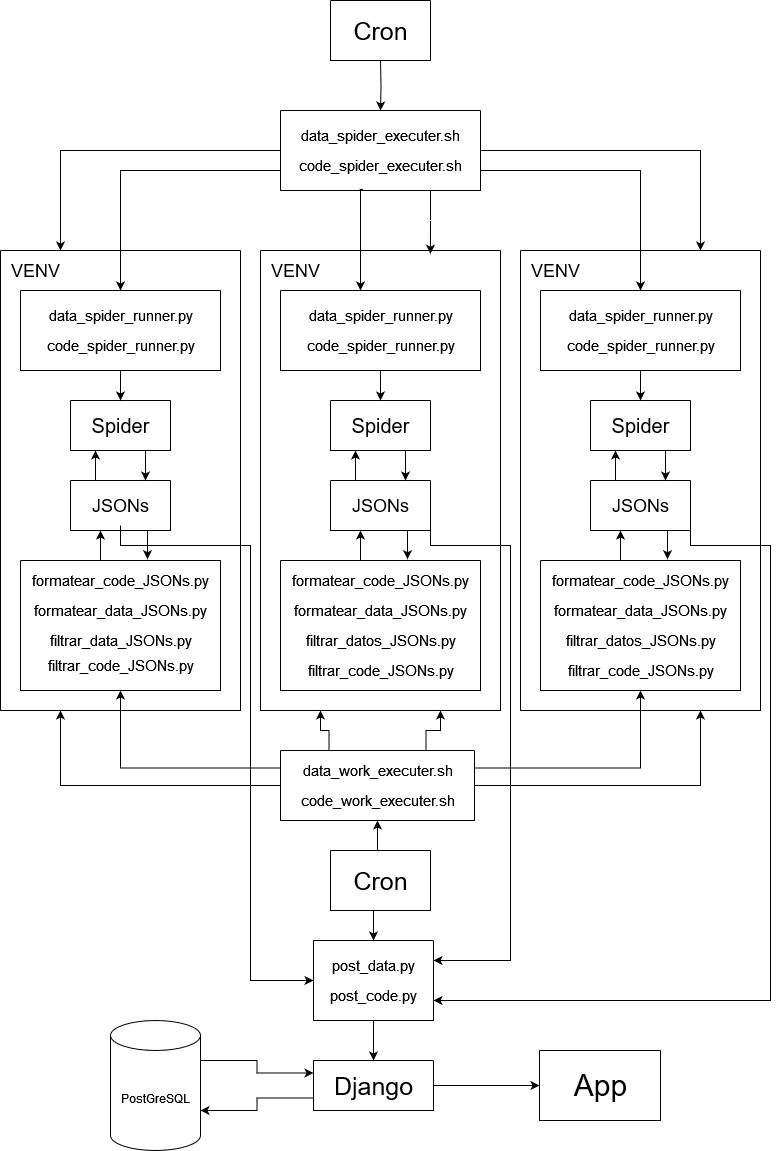
\includegraphics[width=0.7\textwidth]{fig/arquitectura.png}
	\caption[Arquitectura de obtención y tratamiento de datos]{Arquitectura de obtención y tratamiento de datos}
	\label{fig:ej7}
\end{figure}

\subsection{Elementos presentes}

\subsubsection{Entornos virtuales}
Con el fin de que la plataforma sea lo mas fácilmente ampliable se ha decidido que cada Spider disponga de su propio entorno virtual, esto permite añadir dependencias de tal forma que no afecten a el resto de los Scripts presentes, ayudando en la encapsulación de dependencias.
El mayor inconveniente de una plataforma así es la redundancia de código, al ser múltiples entornos independientes es necesario que mucho código sea repetido en cada uno de ellos, cosa que si fuera un único entorno en el que se ejecutara todo, con una clase sobre la que heredar y o una interfaz, seria mucho el código que nos ahorraríamos.
Actualmente la plataforma dispone de cuatro entornos virtuales para cada Spider y un entorno virtual sobre el que ejecutar el servidor de Django.

\subsubsection{Spiders}
Cada Spider representa una web, de tal forma que cada una de ellas obtiene los datos de la web sobre la que se ha diseñado exclusivamente, para poder realizar esta tarea por cada web han sido necesarias varias Spider, aunque de forma simplificada se pueden agrupar por, aquellas que obtienen las estaciones junto con sus códigos y, las de obtención de datos.
De esta forma dividimos las tareas dándonos la posibilidad de ejecutar aquella que mejor nos venga en cada momento.

\subsubsection{Runners}
Runner es la forma en la que han sido nombrados los Scripts cuya función es posibilitar la ejecución en nuestro caso asíncrona de una o múltiples Spiders mediante un único comando.
Es un Script simple en el que una vez dispones de la estructura básica en caso de necesitar añadir o eliminar una Spider solo tienes que agregar o eliminar la Spider en cuestión y ya estaría listo.
A su vez, al añadir un intermediario el comando de ejecución pasa de ser, scrapy crawl nombreSpider por cada Spider que se desea ejecutar, a, python nombreRunner.py facilitando la automatización de ejecución de las Spider.

\subsubsection{Executers}
Aumentado un poco mas la abstracción nos encontramos con los Executers, Scripts en Bash encargados de activar el entorno virtual de la Spider deseada y acto seguido ejecutar su respectivo Runner.
Estos existen (en mayor medida que los Runners) con el fin de ayudar con el mantenimiento de la arquitectura, creando un nuevo intermediario en la cadena de ejecución.
Están diseñados de tal forma que funcionen pasandoles un único argumento representando la web de la que quieres obtener los datos, haciendo que la agregación de nuevas Spiders junto con sus entornos sea tan sencillo como respetar las rutas y nombres predefinidos.

\subsubsection{JSONs}
Este apartado es un conjunto de directorios en los que se van almacenando los JSON obtenidos tras los distintos procesos a los que son sometidos.
Los directorios en cuestión, siguiendo orden de creación para los JSON de datos son los siguientes:
\begin{enumerate}
	\item RawData
	\item ParsedData
	\item RefinedData
	\item OldData
\end{enumerate}
Y los de códigos (estación):
\begin{enumerate}
	\item RawCode
	\item ParsedCode
	\item RefinedCode (TODO)
	\item OldCode (TODO)
\end{enumerate}
El primer nivel es aquel que se obtiene de la llamada con la Spider a la web, devolviendo todos los datos de esta.\newline
El segundo, es obtenido tras ejecutar ya sea formatear\_data\_JSONs.py en caso de querer parsear los datos o formatear\_code\_JSONs.py para los códigos.\newline
El tercero se obtiene tras eliminar la duplicidad de datos en comparación con los ya almacenados en la base de datos mediante la ejecución de filtrar\_data\_JSONs.py.\newline
Finalmente el cuarto es el subproducto obtenido tras la comparación, tomando el fichero original ya formateado y cambiándole de directorio y el nombre de tal forma que se distinga del resto de ficheros.\newline

\subsubsection{Posts}
Estos Scripts son los encargado de enviar los datos mediante un Post Request al servidor Django.





